% !TeX root = ../thuthesis-example.tex

\chapter{数据集分析与对比}
\section{开源数据集}
\subsection{UNSW-NB15}
UNSW-NB15 数据集是 2015 年澳大利亚网络安全中心使用 IXIA Perfect Storm工具模拟网络环境流量而生成的一个数据集。相比于 KDD99 是一个更新的数据集,因此更能代表真实的网络流量。UNSW-NB15 数据集中包括 100GB的.pcap 格式的原始网络流量,同时还有 4 个经过特征提取的 csv 文件,分别是UNSW-NB15\_1.csv  、 UNSW-NB15\_2.csv 、 UNSW-NB15\_3.csv  和   UNSW-NB15\_4.csv,一共是 2540044 条数据,同时该数据集提出了与 KDD99 较为不同的特征,这些特征更为符合当前的网络协议模式。 UNSW-NB15 一共包含有 10 个分类,一个正常类别和 9 个攻击类别,其具体描述和类别数目如下表所示: 
% 表 3.2 攻击类型描述和数目 

% \flushleft{

    \begin{table}[H]
        \begin{tabular}{|p{0.1\textwidth}<{\centering} |p{0.7\textwidth}<{\centering} |p{0.1\textwidth}<{\centering}|}
        % \begin{tabular}{lp{3cm}p{9cm}p{3cm}}
        \toprule 
        类别 & 类别描述                                                                       & 样本数量    \\ \midrule 
        Normal  & 正常流量                                                                       & 2218761 \\ \hline
        Fuzzers & 攻击者从命令行或以报文的形式发送大量随机生成的输入序列。攻击者试图发现操作系统、程序或网络中的安全漏洞,并使这些资源挂起一段时间,甚至可以使它们崩溃 & 24246   \\ \hline
        Analysis & 这类攻击是指通过端口扫描、恶意 web 脚本
    (如 HTML 文件渗透)和发送垃圾邮件等各种
    方式渗透到 web 应用程序的各种入侵等。 & 2677 \\ \hline
    Backdoor & 这类攻击中攻击者可以绕过正常的身份验证
    并获得对系统的未授权远程访问。黑客利用
    后门程序安装恶意文件,修改代码或获得对
    系统或数据的访问。 &
    2329 \\ \hline
    DoS & 攻击者使某些计算或内存资源过于繁忙或占
    据全部资源而无法处理合法请求或者拒绝合
    法用户对计算机的访问。 &
    16353 \\ \hline
    Exploit & 利用操作系统或软件中的软件漏洞、漏洞或
    故障进行入侵的行为。攻击者利用软件的知
    识发动攻击,意图对系统造成危害。 &
    44525 \\ \hline
    Generic & 针对密码系统的攻击,试图破坏安全系统的
    密钥。它独立于密码系统的实现细节。不考
    虑块密码的结构。例如,生日攻击是一种将
    哈希函数视为黑盒的通用攻击。 &
    215481 \\ \hline
    Reconnaissance & 为了绕过目标计算机网络的安全控制而收集
    其信息的攻击。它可以被定义为一个探针,
    是发起进一步攻击的初步步骤。攻击者使用
    各种扫描手段来收集系统信息。在收集到足
    够的信息后,可以发起后续的攻击。 &
    13987 \\ \hline
    Shellcode & Shellcode 作为负载在目标机器执行,来挖掘
    该软件的漏洞。之所以称作 Shellcode 是因为
    启动了受到攻击者控制的命令行 shell。 &
    1511 \\ \hline
    Worm & 蠕虫是一种恶意程序或恶意软件,它可以复
    制自己并传播到其他计算机。 &
    174 \\  
        \bottomrule
        \end{tabular}
        \end{table}



 
UNSW-NB15 数据集一共包含 47 个特征,其中时间戳,IP 地址,端口号等特
征对训练无用,因此有效的特征一共 41 个。 
下面对这些特征做一个概括的说明。按照数据集作者的思路,可以分为基本
特征,内容特征,时间特征和额外生成的特征这几类。这里从另外一种思路进行
重新归类可以分为以下几类。


\begin{table}[H]
    \caption{与协议相关的特征}
    \centering
    \begin{tabular}{|l|l|}
    \hline
    特征名称                  & 特征描述                      \\ \hline
    proto                 & 传输层协议                     \\ \hline
    service               & 应用层协议                     \\ \hline
    sttl                  & 从源发出的报文的 time to live     \\ \hline
    dttl                  & 从目的发出的报文的 time to live 字段 \\ \hline
    stcpb                 & 源 tcp 报文的初始序列号            \\ \hline
    dtcpb                 & 目的 tcp 报文的初始序列号           \\ \hline
    swin                  & 源 tcp 报文的窗口字段             \\ \hline
    dwin                  & 目的 tcp 报文的窗口字段            \\ \hline
    res\_bdy\_len         & http 响应内容的长度              \\ \hline
    ct\_flw\_http\_method & 会话中 http 方法字段的计数          \\ \hline
    is\_ftp\_login        & 是否有 ftp 的登录               \\ \hline
    ct\_ftp\_cmd          & 会话中 ftp 命令的计数             \\ \hline
    trans\_depth          & http 服务的连接深度              \\ \hline
    \end{tabular}
    \end{table}

\begin{table}[H]
    \caption{与时间相关的特征}
    \centering
    \begin{tabular}{|l|l|}
    \hline
    dur     & 会话的持续时间                        \\ \hline
    tcprtt  & tcp 三次握手的 rtt(round trip time) \\ \hline
    synack  & 第一次发送到确认的时间                    \\ \hline
    ackdat  & 确认之后返回的时间                      \\ \hline
    sintpkt & 源报文的间隔时间的平均值                   \\ \hline
    dintpkt & 目的报文间隔时间的平均值                   \\ \hline
    sjit    & 源报文间隔时间的标准差(jitter)            \\ \hline
    djit    & 目的报文间隔时间的标准差                   \\ \hline
    sload   & 源报文的吞吐量                        \\ \hline
    dload   & 目的报文的吞吐量                       \\ \hline
    \end{tabular}
    \end{table}

    \begin{table}[H]
        \caption{与报文大小相关的特征}
        \centering
        \begin{tabular}{|l|l|}
        \hline
        sbytes  & 会话中从源发出的总字节数  \\ \hline
        dbytes  & 会话中从目的发出的总字节数 \\ \hline
        smeansz & 会话中源报文的平均大小   \\ \hline
        dmeansz & 会话中目的报文的平均大小  \\ \hline
        spkts   & 会话中源的报文总数     \\ \hline
        dpkts   & 会话中目的报文总数     \\ \hline
        \end{tabular}
        \end{table}

\begin{table}[H]
    \caption{与连接状态相关的特征}
    \centering
    \begin{tabular}{|l|l|}
    \hline
    sloss & 源的丢包数和重传数之和  \\ \hline
    dloss & 目的的丢包数和重传数之和 \\ \hline
    state & 会话的状态和相应的协议  \\ \hline
    \end{tabular}
    \end{table}

\begin{table}[H]
    \caption{额外构造的特征}
    \centering
    \begin{tabular}{|l|l|}
    \hline
    ct\_srv\_src                & 根据最后一条报文的时间排序,每 100 条记录中源ip 与服务都相同的会话计数(下面省略每 100 条)  \\ \hline
    ct\_srv\_dst                & 目的 IP 与服务都相同的会话计数         \\ \hline
    ct\_dst\_ltm                & 目的 IP 相同的会话计数             \\ \hline
    ct\_src\_ltm                & 源 IP 相同的会话计数              \\ \hline
    ct\_src\_dport\_ltm         & 源 IP 和目的端口都相同的会话计数        \\ \hline
    ct\_dst\_sport\_ltm         & 目的 IP 和源端口都相同的会话计数        \\ \hline
    ct\_dst\_src\_ltm           & 目的 IP 和源 IP 都相同的会话计数      \\ \hline
    ct\_state\_ttl              & 对于每一个状态,ttl 值的范围          \\ \hline
    is\_sm\_ips\_ports          & 源 ip 与目的 ip,源端口和目的端口是否都相同 \\ \hline
    \end{tabular}
    \end{table}
 
可以看到,UNSW-NB15 数据集大多数特征都有较为清晰的定义,因此可以
用做流量数据特征提取的标准。 

\subsection{CICIDS2017}
CICIDS数据集特征介绍如下:(修改成跨页表格)


List of extracted features and descriptions: \\

% \begin{longtable}{cc}
%     \begin{tabular}
%       abc & dfg
% \end{tabular}
% \end{longtable}


\begin{table}[H]
    \caption{packet大小相关的特征}
    \centering
    \begin{tabular}{|l|l|}
    \hline
    total Length of Fwd Packet	& 发送方packet总长度 \\
    total Length of Bwd Packet	& 接收方packet总长度 \\
    Fwd Packet Length Min 		& 发送方packet最小长度 \\
    Fwd Packet Length Max 		& 发送方packet最大长度 \\
    Fwd Packet Length Mean		& 发送方packet平均长度 \\
    Fwd Packet Length Std		& 发送方packet长度标准差 \\
    Bwd Packet Length Min		& 接收方packet最小长度 \\
    Bwd Packet Length Max		& 接收方packet最大长度 \\
    Bwd Packet Length Mean		& 接收方packet平均长度 \\
    Bwd Packet Length Std		& 接收方packet长度标准差 \\
    \hline
    \end{tabular}
    \end{table}

\begin{table}[H]
    \caption{时间相关的特征}
    \centering
    \begin{tabular}{|l|l|}
    \hline
    Flow Bytes/s		&	bps \\
    Flow Packets/s		&	pps  \\
    Flow IAT Mean		&	一条流中包平均间隔时间 \\
    Flow IAT Std		&	一条流中包间隔时间的标准差 \\
    Flow IAT Max		&	一条流中两个packet最大间隔时间 \\
    Flow IAT Min		&	一条流中两个packet最小间隔时间 \\
    Fwd IAT Min			&发送方两个packet最小间隔时间\\
    Fwd IAT Max			&发送方两个packet最大间隔时间 \\
    Fwd IAT Mean		&	发送方两个packet平均间隔时间 \\
    Fwd IAT Std			&发送方两个packet间隔时间的标准差 \\
    Fwd IAT Total   	&	发送方两个packet总间隔时间\\
    Bwd IAT Min			&接收方两个packet最小间隔时间\\
    Bwd IAT Max			&接收方两个packet最大间隔时间\\
    Bwd IAT Mean		&	接收方两个packet平均间隔时间 \\
    Bwd IAT Std			&接收方两个packet间隔时间的标准差 \\
    Bwd IAT Total		&	接收方两个packet总间隔时间 \\  
    \hline
    \end{tabular}
    \end{table}

    
Flow duration  单条流持续时间/微秒 \\
total Fwd Packet		发送方packet数量 \\
total Bwd packets		接收方packet数量 \\
% total Length of Fwd Packet	发送方packet总长度 \\
% total Length of Bwd Packet	接收方packet总长度 \\
% Fwd Packet Length Min 		发送方packet最小长度 \\
% Fwd Packet Length Max 		发送方packet最大长度 \\
% Fwd Packet Length Mean		发送方packet平均长度 \\
% Fwd Packet Length Std		发送方packet长度标准差 \\
% Bwd Packet Length Min		接收方packet最小长度 \\
% Bwd Packet Length Max		接收方packet最大长度 \\
% Bwd Packet Length Mean		接收方packet平均长度 \\
% Bwd Packet Length Std		接收方packet长度标准差 \\
% Flow Bytes/s			bps \\
% Flow Packets/s			pps  \\
% Flow IAT Mean			一条流中包平均间隔时间 \\
% Flow IAT Std			一条流中包间隔时间的标准差 \\
% Flow IAT Max			一条流中两个packet最大间隔时间 \\
% Flow IAT Min			一条流中两个packet最小间隔时间 \\
% Fwd IAT Min			发送方两个packet最小间隔时间\\
% Fwd IAT Max			发送方两个packet最大间隔时间 \\
% Fwd IAT Mean			发送方两个packet平均间隔时间 \\
% Fwd IAT Std			发送方两个packet间隔时间的标准差 \\
% Fwd IAT Total   		发送方两个packet总间隔时间\\
% Bwd IAT Min			接收方两个packet最小间隔时间\\
% Bwd IAT Max			接收方两个packet最大间隔时间\\
% Bwd IAT Mean			接收方两个packet平均间隔时间 \\
% Bwd IAT Std			接收方两个packet间隔时间的标准差 \\
% Bwd IAT Total			接收方两个packet总间隔时间 \\
Fwd PSH flags			发送方PSH标志位出现次数(0 for UDP) \\
Bwd PSH Flags			接收方PSH标志位出现次数(0 for UDP)\\
Fwd URG Flags			发送方URG标志位出现次数(0 for UDP) \\
Bwd URG Flags			接收方URG标志位出现次数(0 for UDP) \\
Fwd Header Length		发送方header占用的总字节数 \\
Bwd Header Length		接受方header占用的总字节数 \\
FWD Packets/s			发送方pps \\
Bwd Packets/s			接收方pps \\
Packet Length Min 		packet最小长度 \\
Packet Length Max		packet最大长度 \\
Packet Length Mean 		packet平均长度 \\
Packet Length Std		packet长度标准差 \\
Packet Length Variance  	packet长度方差 \\
FIN Flag Count 			FIN标志位出现次数 \\
SYN Flag Count 			SYN标志位出现次数 \\
RST Flag Count 			RST标志位出现次数 \\
PSH Flag Count 			PUSH标志位出现次数 \\
ACK Flag Count 			ACK标志位出现次数 \\
URG Flag Count 			URG标志位出现次数 \\
CWR Flag Count 			CWR标志位出现次数 \\
ECE Flag Count 			ECE标志位出现次数 \\
down/Up Ratio			下载/上传比 \\
Average Packet Size 		packet平均大小 \\
Fwd Segment Size Avg 		发送方数据块平均大小?\\
Bwd Segment Size Avg 		接收方数据块平均大小?\\
Fwd Bytes/Bulk Avg		Average number of bytes bulk rate in the forward direction \\
Fwd Packet/Bulk Avg		Average number of packets bulk rate in the forward direction \\
Fwd Bulk Rate Avg 		Average number of bulk rate in the forward direction \\
Bwd Bytes/Bulk Avg		Average number of bytes bulk rate in the backward direction \\
Bwd Packet/Bulk Avg 		Average number of packets bulk rate in the backward direction \\
Bwd Bulk Rate Avg		Average number of bulk rate in the backward direction \\
Subflow Fwd Packets		The average number of packets in a sub flow in the forward direction \\
Subflow Fwd Bytes		The average number of bytes in a sub flow in the forward direction \\
Subflow Bwd Packets		The average number of packets in a sub flow in the backward direction \\
Subflow Bwd Bytes		The average number of bytes in a sub flow in the backward direction \\
Fwd Init Win bytes		The total number of bytes sent in initial window in the forward direction \\
Bwd Init Win bytes		The total number of bytes sent in initial window in the backward direction \\
Fwd Act Data Pkts		Count of packets with at least 1 byte of TCP data payload in the forward direction \\
Fwd Seg Size Min		Minimum segment size observed in the forward direction \\
Active Min			Minimum time a flow was active before becoming idle \\
Active Mean			Mean time a flow was active before becoming idle \\
Active Max			Maximum time a flow was active before becoming idle \\
Active Std			Standard deviation time a flow was active before becoming idle \\
Idle Min			Minimum time a flow was idle before becoming active \\
Idle Mean			Mean time a flow was idle before becoming active \\
Idle Max			Maximum time a flow was idle before becoming active \\
Idle Std			Standard deviation time a flow was idle before becoming active \\

\section{校园网真实数据集}

校园网规模巨大,每天有海量的数据,这给我们的分析带来了很多困难。
校园网的原始数据为抓包(Packet Capture,pcap)流量,如下图~\ref{fig:wireshark}所示,包含每个数据包的详细信息,如五元组、报文内容等。

\begin{figure}
    \centering
    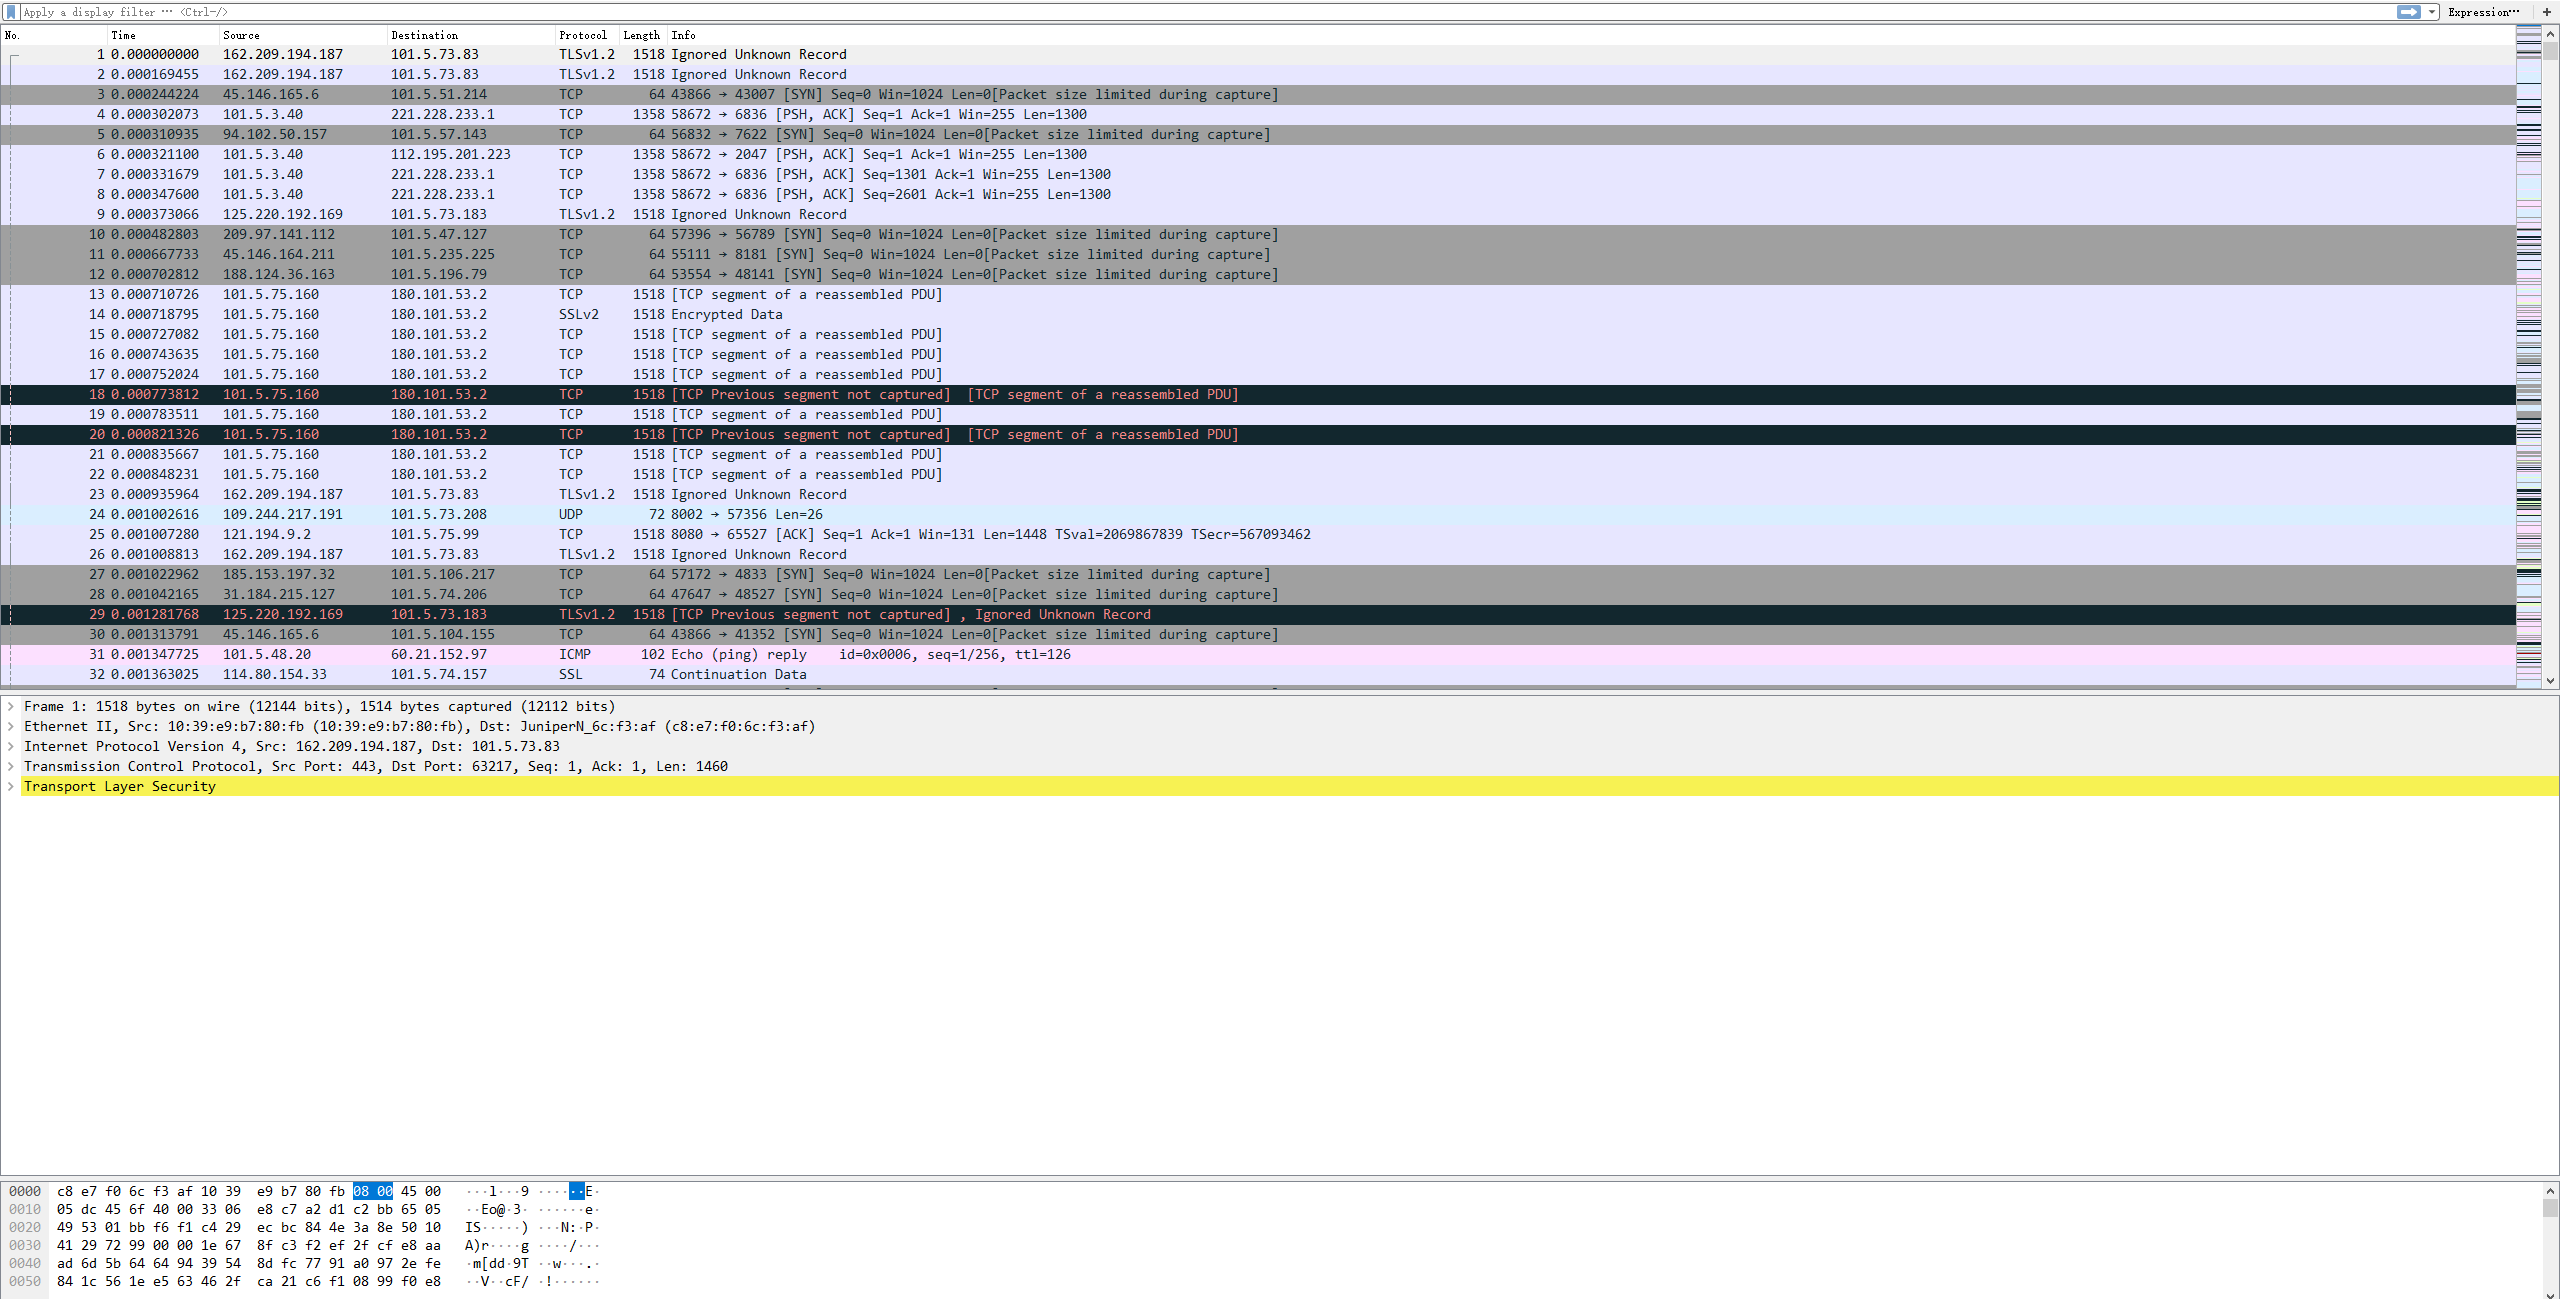
\includegraphics[scale=0.2]{wireshark流量图.png}
    % 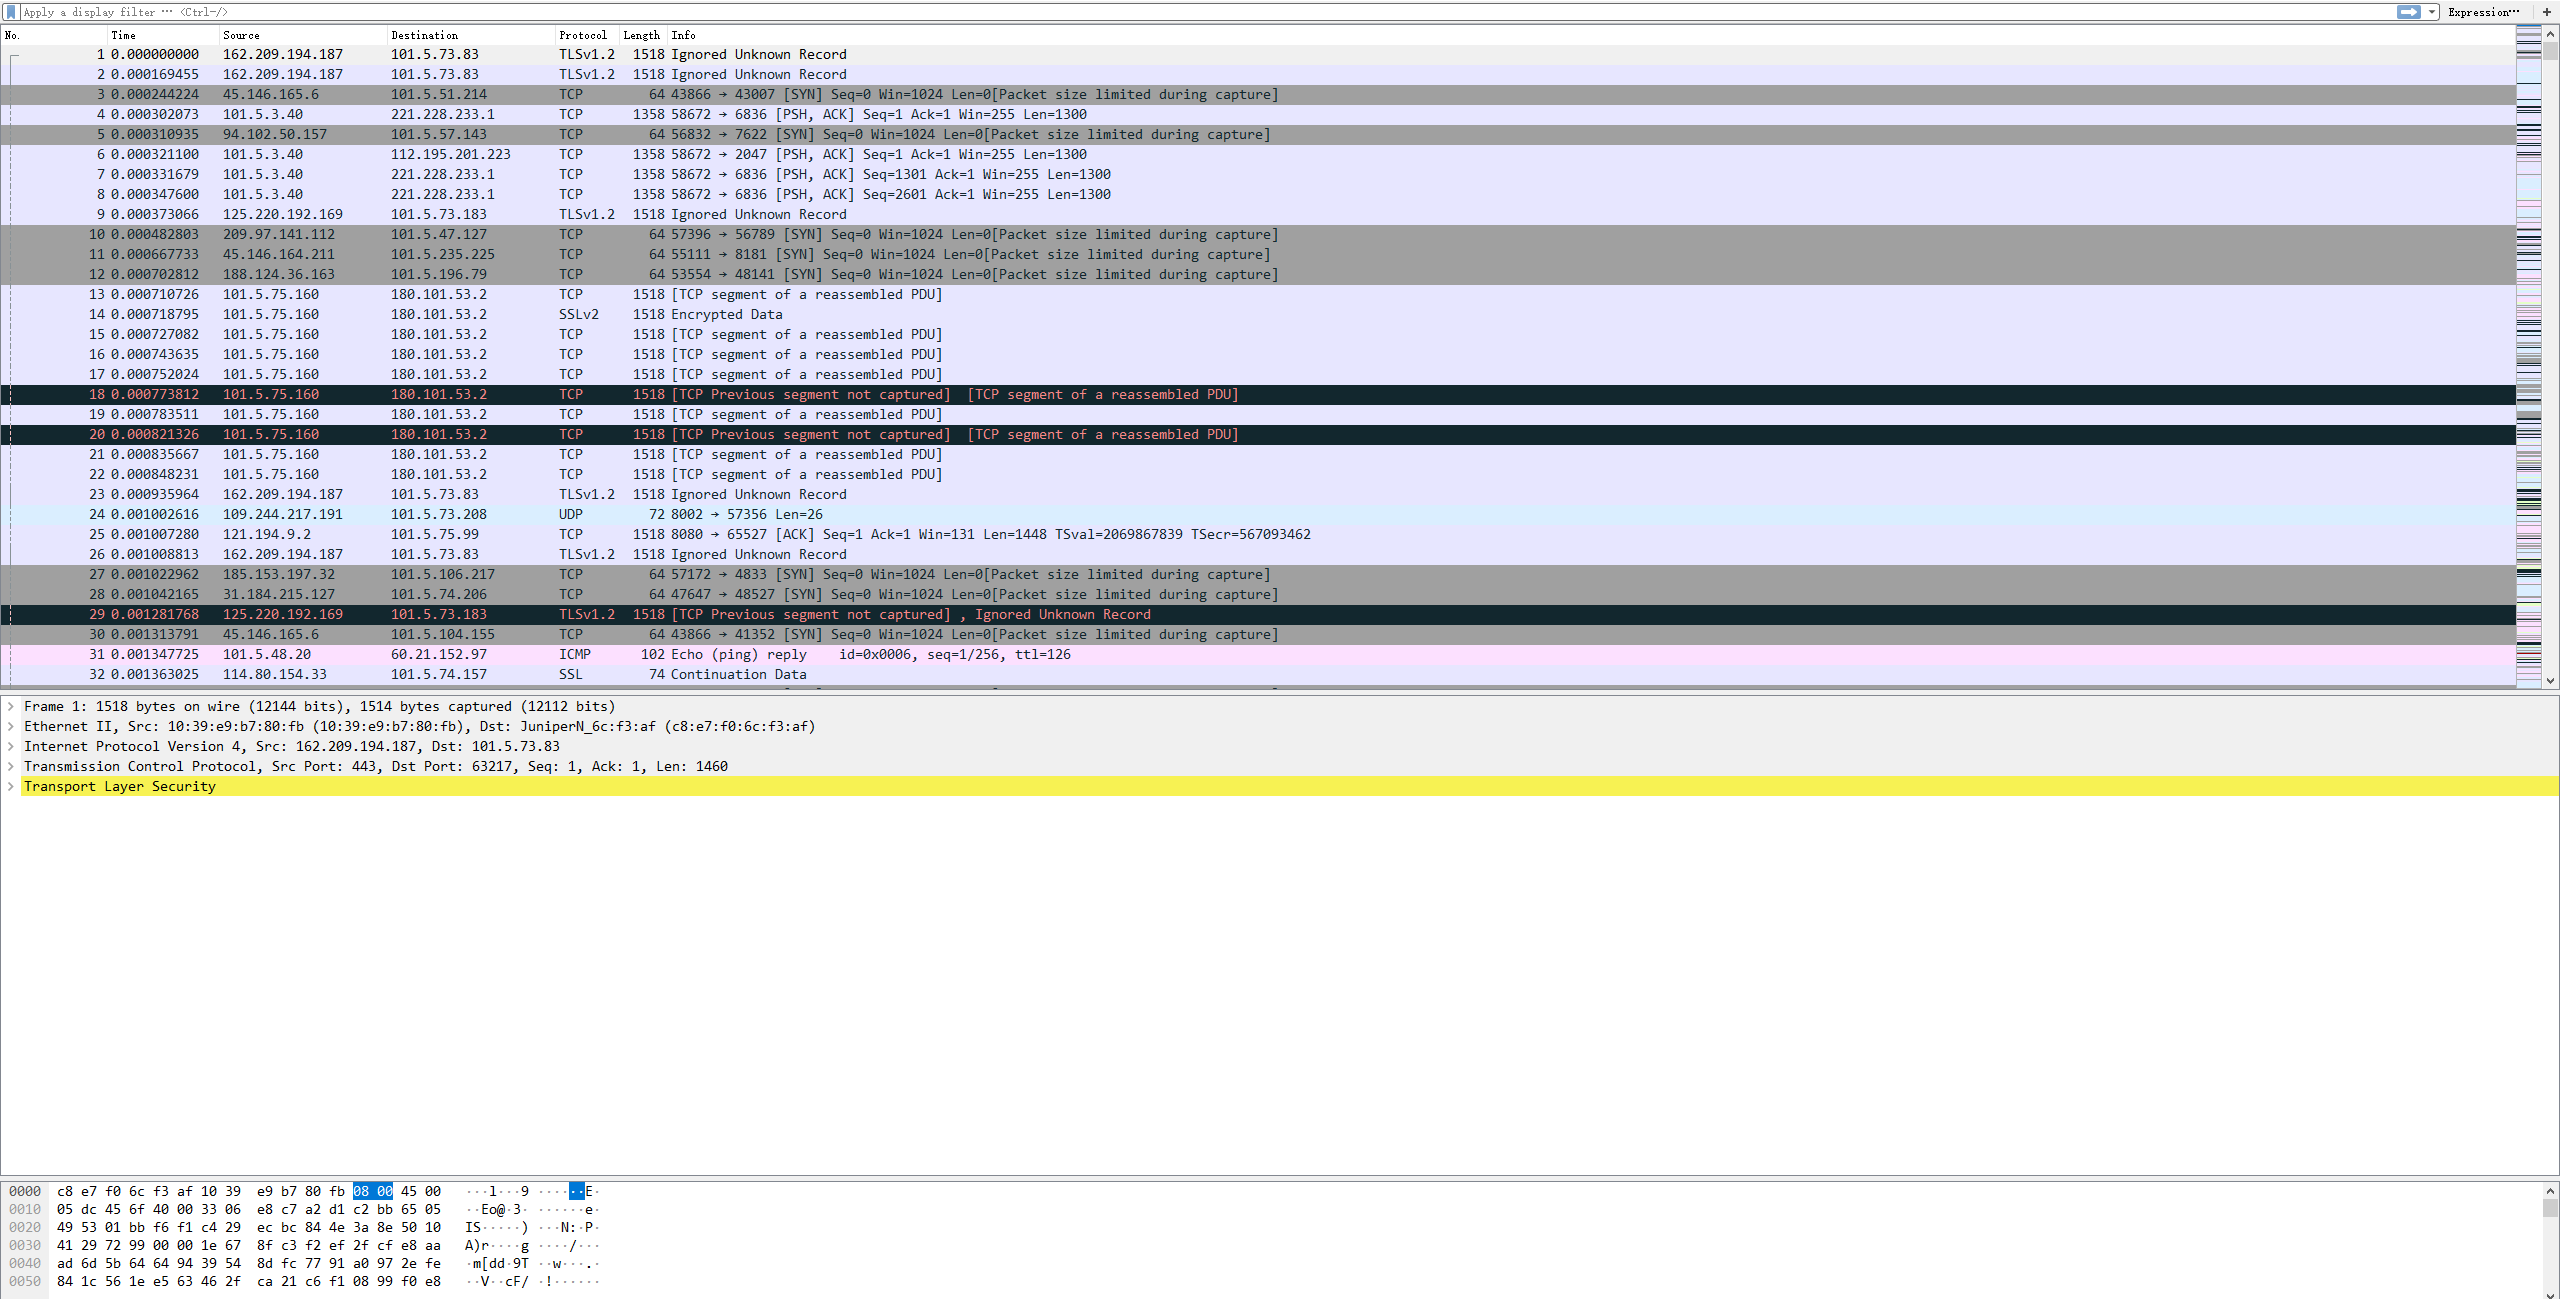
\includegraphics[width=0.6\linewidth]{wireshark流量图.png}
    \caption{流量数据示意图}
    \label{fig:wireshark}
  \end{figure}

  对于机器学习模型来说,通常
  不是直接对原始的流量进行检测,而是通过对流量提取特征,得到样本的特征向
  量后进行检测和分类。因此数据集的制作流程如图所示:
  \begin{figure}
    \centering
    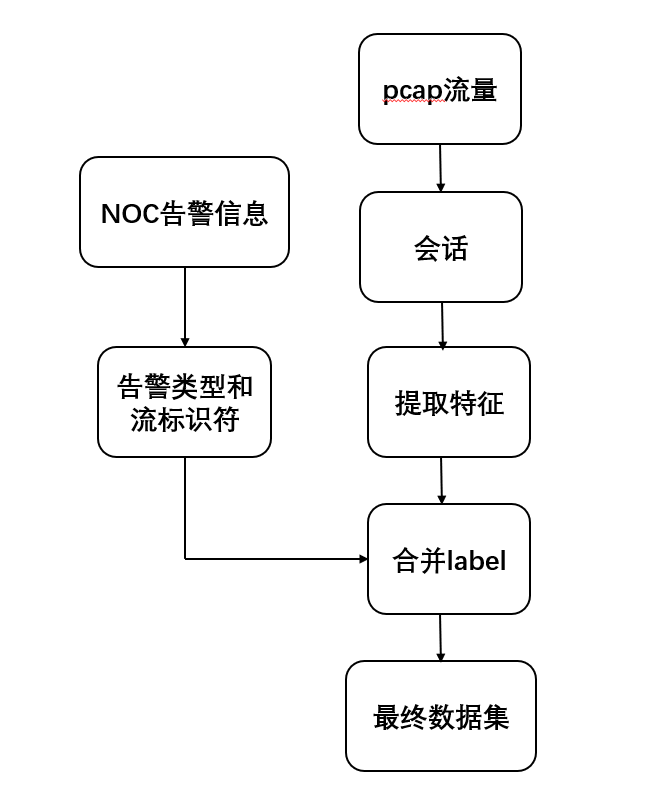
\includegraphics[scale=0.6]{流量数据集制作流程.png}
    % 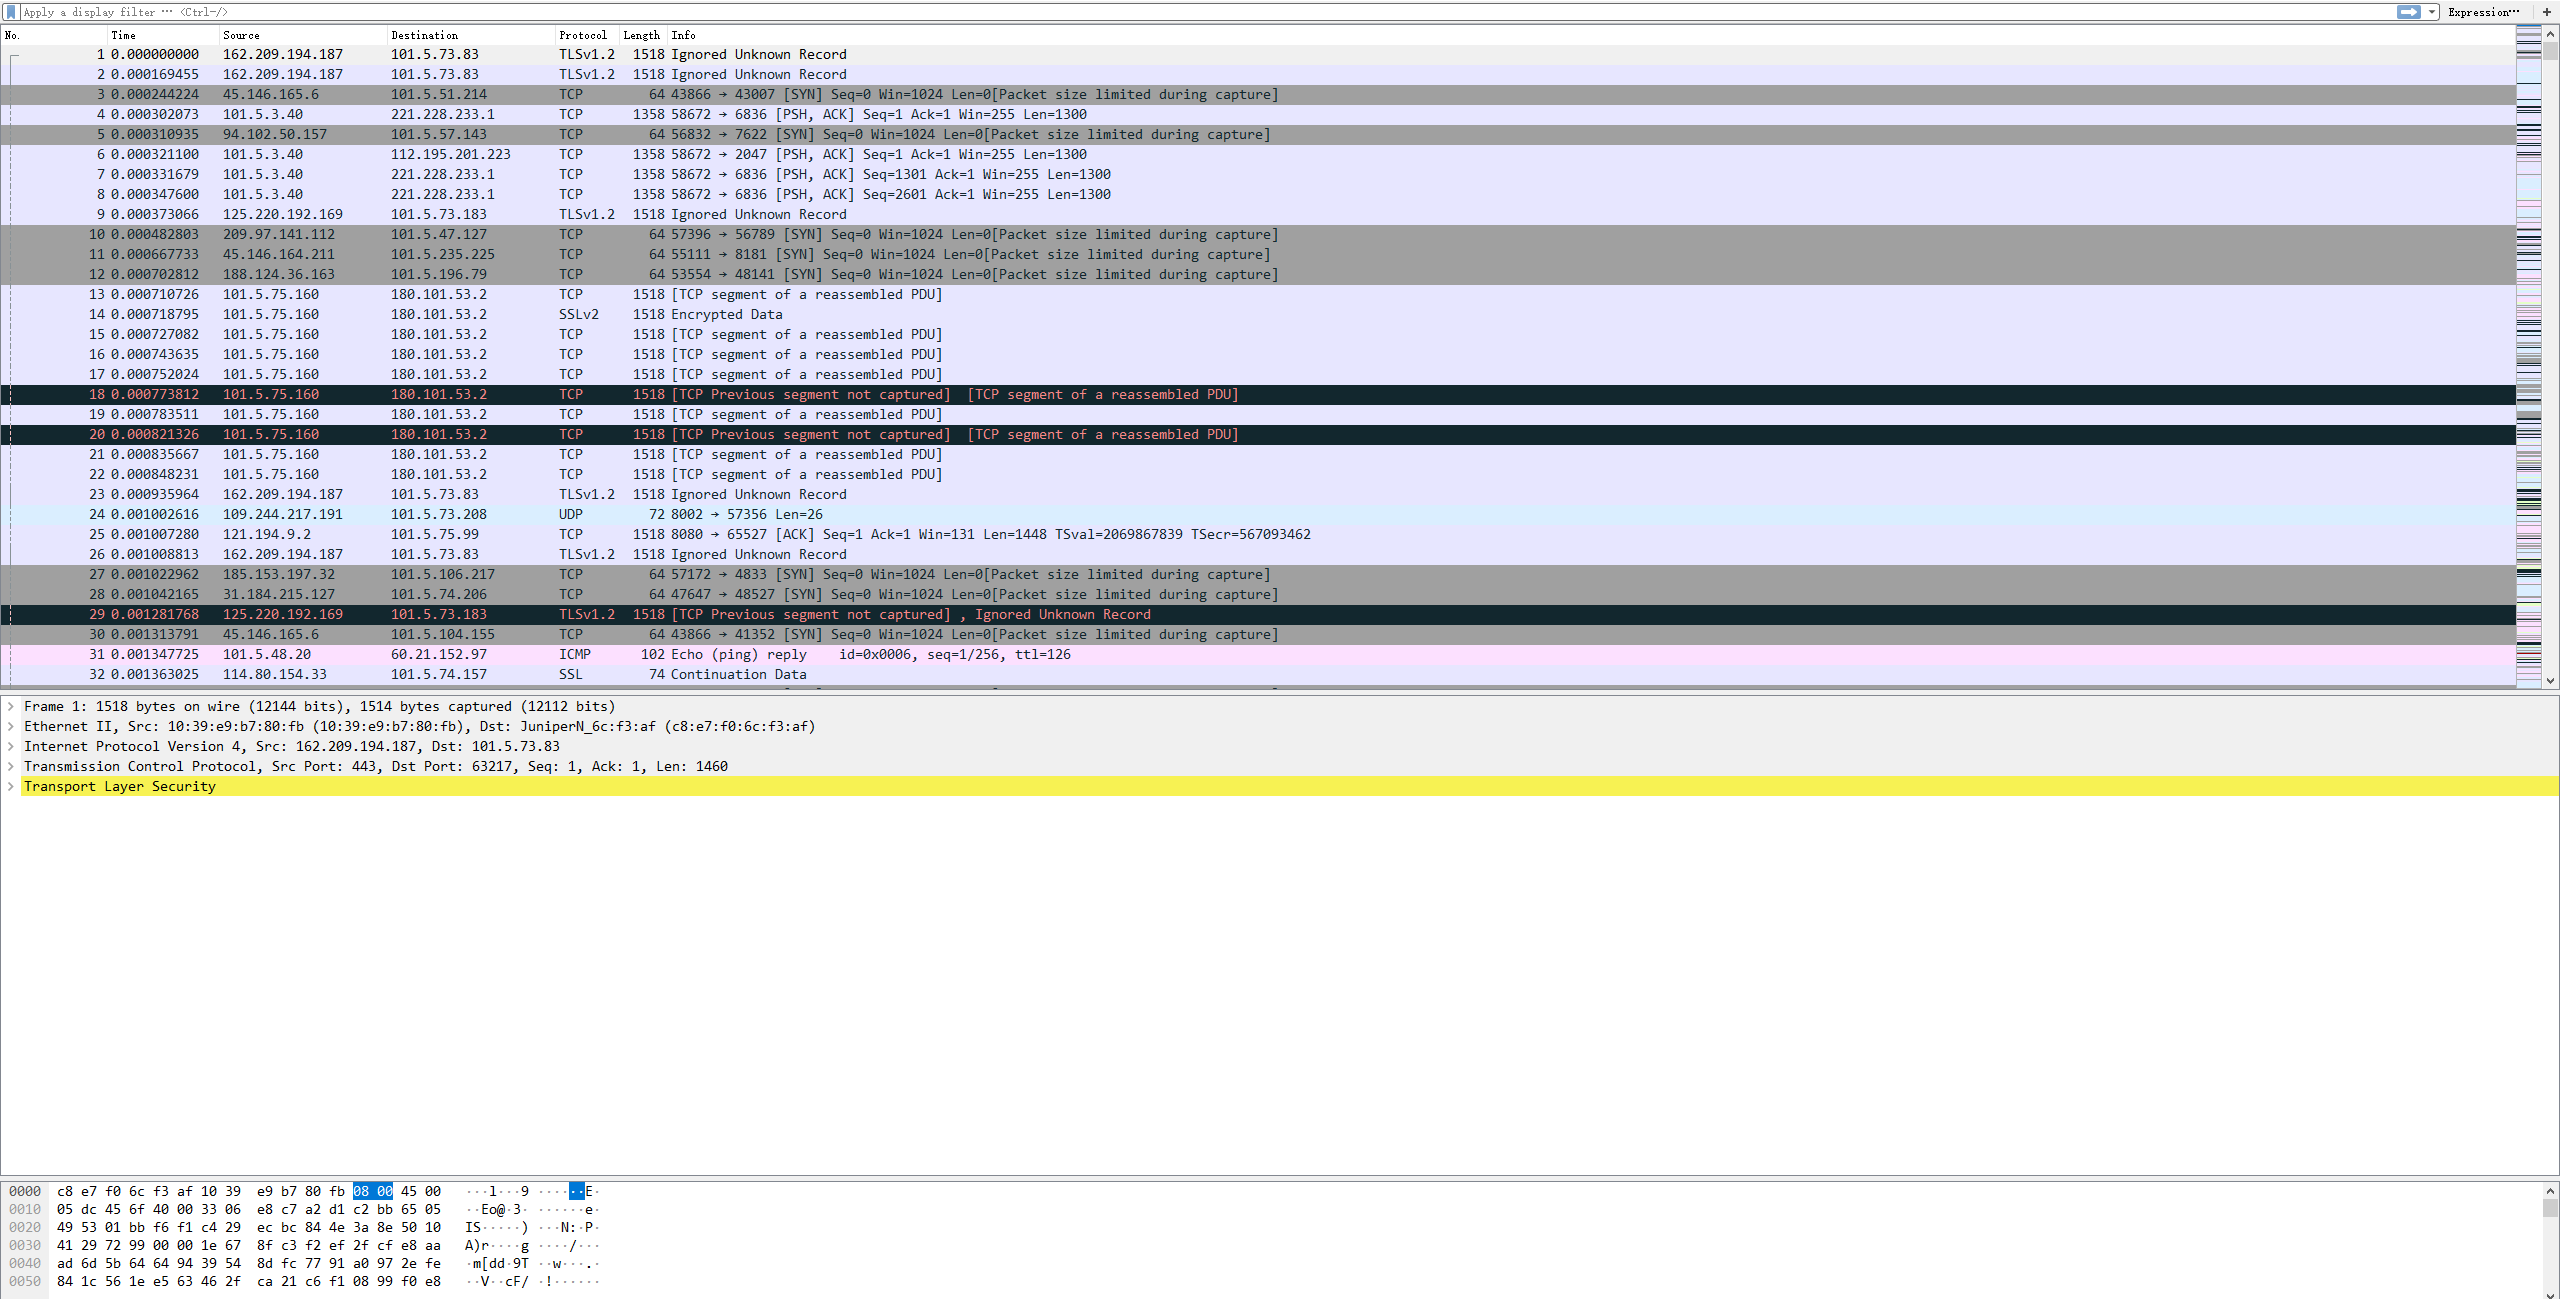
\includegraphics[width=0.6\linewidth]{wireshark流量图.png}
    \caption{流量数据集制作流程}
    \label{fig:flow}
  \end{figure}


经过第5章的特征提取模块,我们得到了特征数据集,但是由于缺乏标注,该数据集无法进行训练以及验证。因此为了得到可进行训练的有效数据集,我们还需要对特征数据集进行标注。标注数据是根据现有的NOC平台得到,需要进行数据清洗、数据预处理等步骤。下图为NOC平台的数据样例。
\begin{figure}
    \centering
    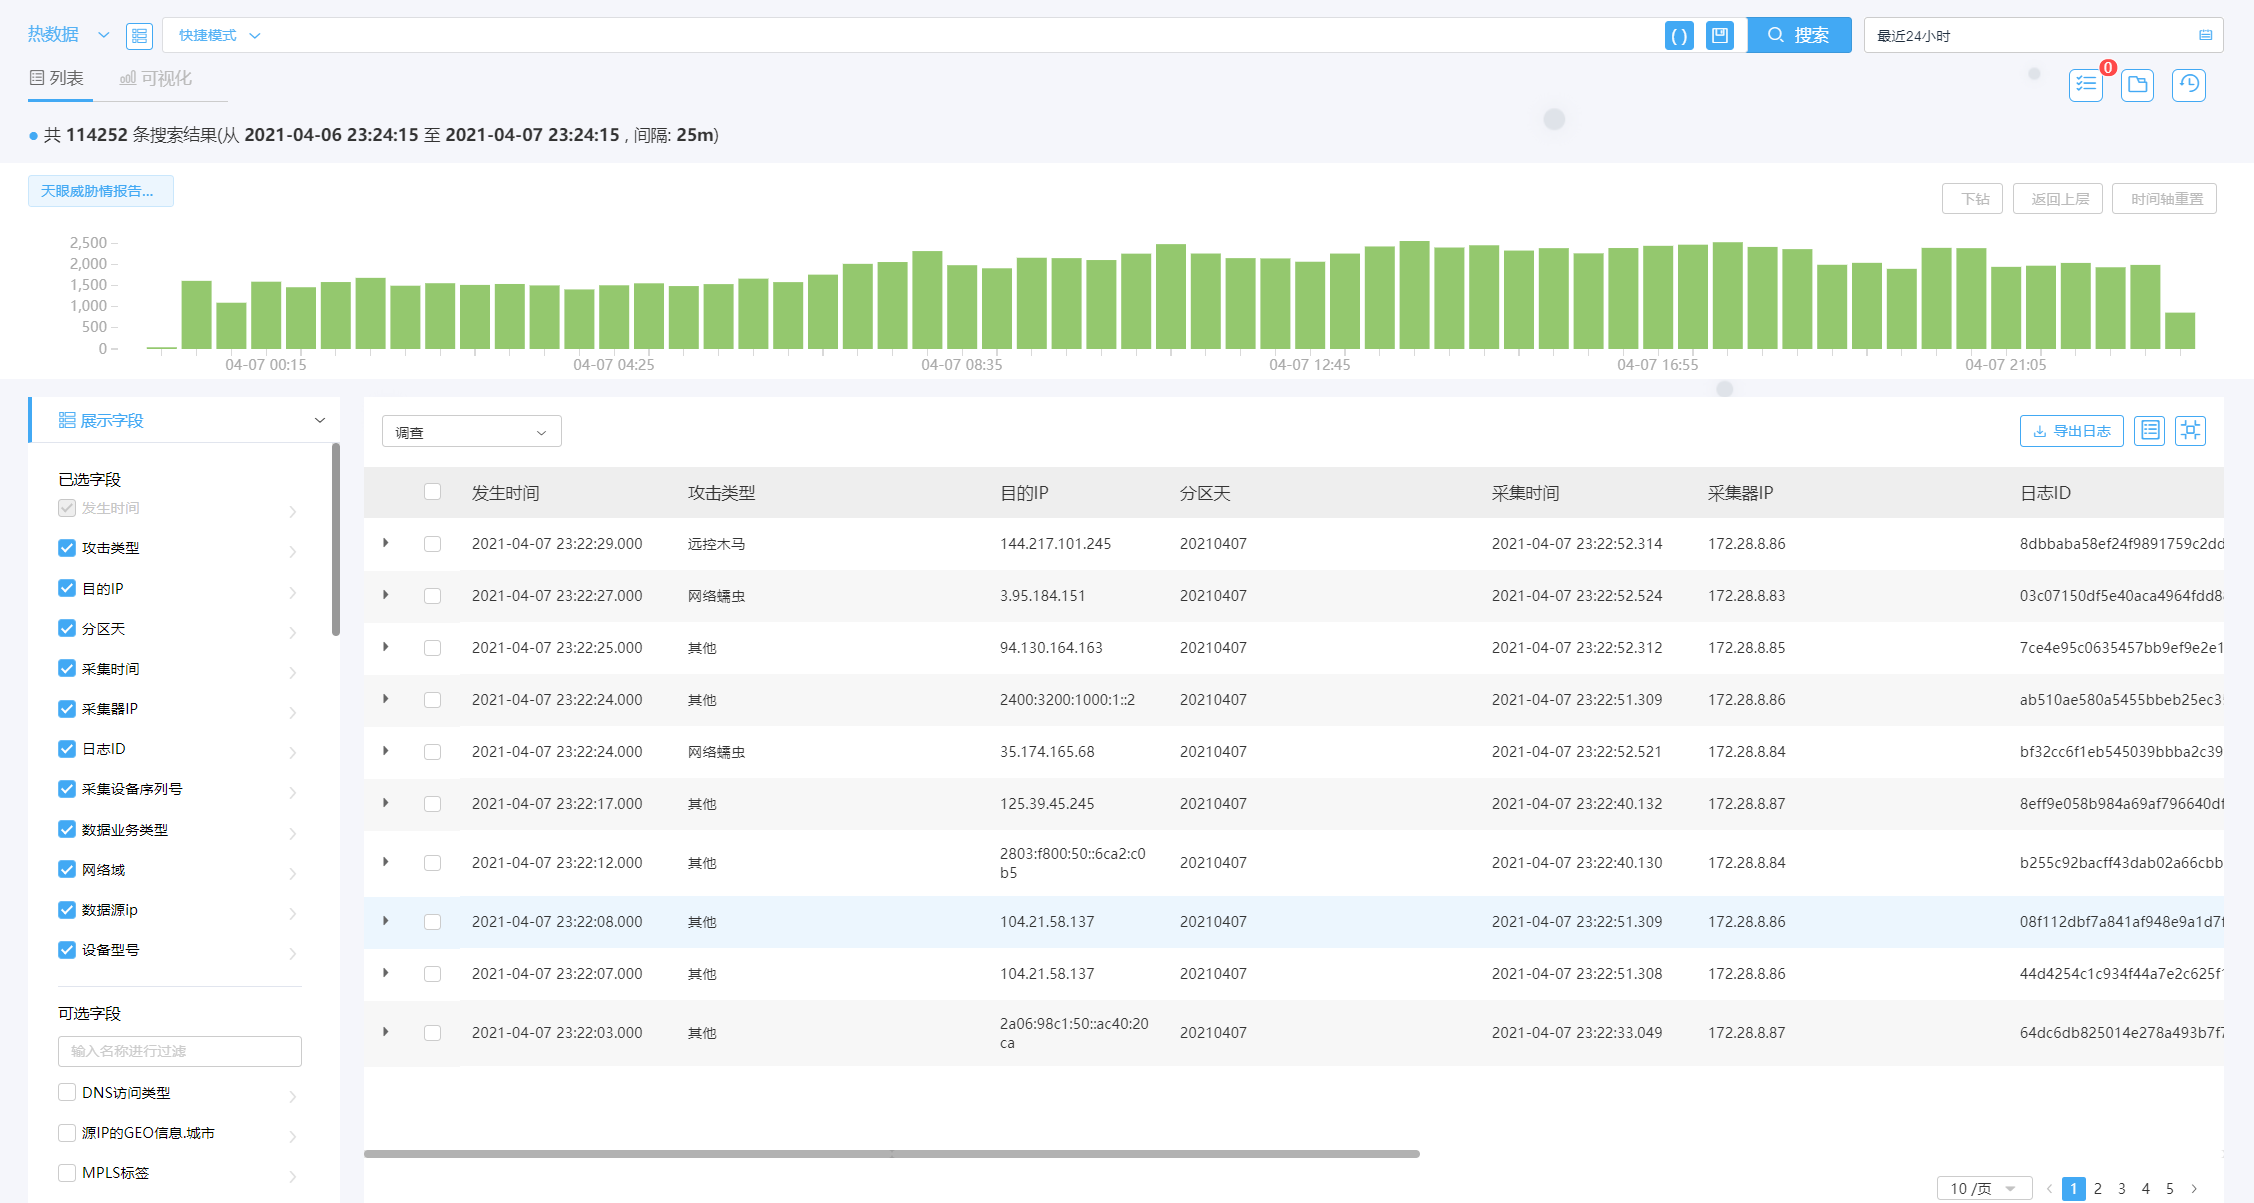
\includegraphics[scale=0.6]{NOC平台.png}
    % 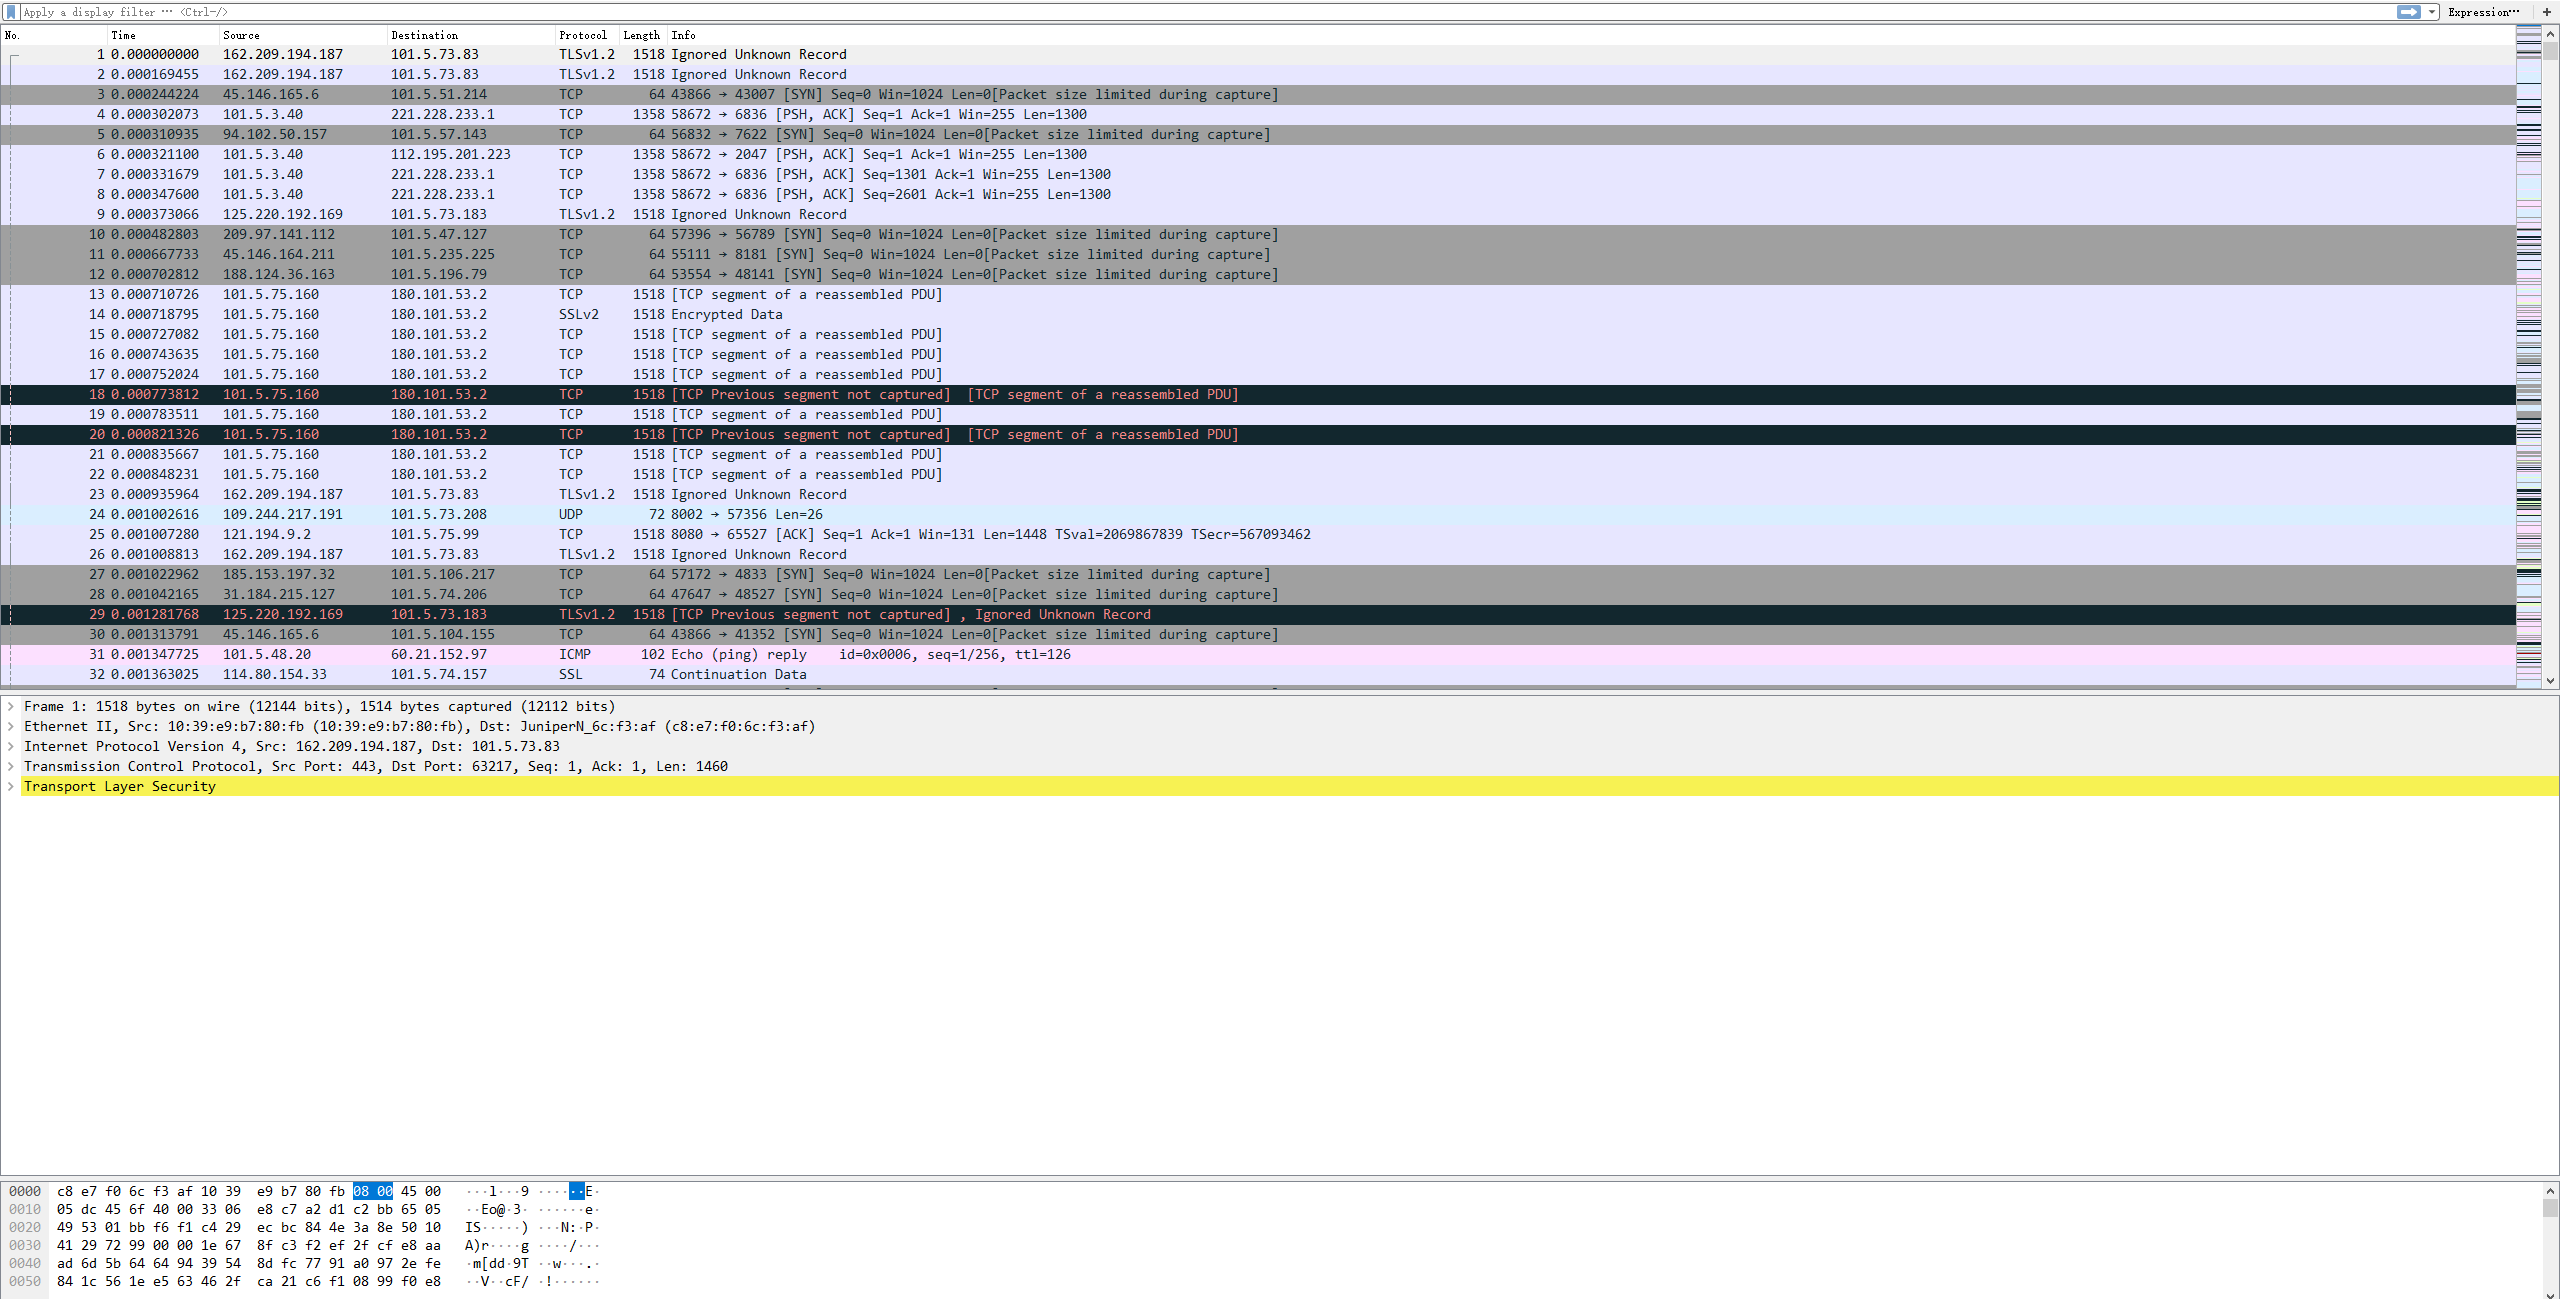
\includegraphics[width=0.6\linewidth]{wireshark流量图.png}
    \caption{NOC平台数据样例}
    \label{fig:NOC}
  \end{figure}

\section{数据预处理及评价指标}
数据预处理阶段,首先对数据进行数据清洗,消除不必要的噪声数据。后续操作总结如下:

1. 删除套接字信息:由于原始数据集包含网络中源主机和目标主机的 IP 地址和端口号,因此删除这些信息以提供无偏检测非常重要,使用这些信息可能会导致对该套接字信息的过度训练。

2. 删除空格:数据集中的一些多类标签包含空格。由于实际值不同于同一
类中其他元组的标签,因此这些空白会导致不同的类。

3. 标签编码:数据集中的多个类标签都有攻击的名称,即字符串值。因此
这些值编码成数值是很重要的,分类器就可以学习每个元组所属的类号。

4. 数据规范化:数据集中的数值数据属于不同的范围,这给分类器在训练
过程中补偿这些差异带来了一些挑战。因此,规范化每个属性中的值很重要,这
样,每个属性中的最小值为零,而最大值为一。这为分类器提供了更均匀的值,
同时保持了每个属性值之间的相关性。

在实验中,本论文使用四个指标来评估模型的性能:准确率,精确度,召回
率和 $F1-score$。对于一个数据样本检测的结果可分为下面的结果:

1. TP:入侵网络流量被入侵检测正确的识别为入侵网络流量

2. TN:正常网络流量被入侵检测正确的识别为正常网络流量

3. FN:入侵网络流量被入侵检测错误的识别为正常网络流量

4. FP:正常网络流量被入侵检测错误的识别成入侵网络流量

论文使用下面的方法去评估我们提出方法的性能:
准确率(Accuracy): 预测正确的样本的数量与所有被预测样本数量的比值,
公示如 所示。
\begin{equation}
    Accuracy = \frac{TP + TN}{TP + TN + FN + FP}
\end{equation}

精确度(Precision): 这个指标于分类器衡量的被错误分类的数量所惩罚的
正确分类的数量,公示如 所示
\begin{equation}
    Precision = \frac{TP}{TP + FP}
\end{equation}
召回率(Recall): 针对样本而言的表示的是数据正样本中有多少被预测正
确。这种度量反映了分类器检测网络攻击的能力,公示如 (5.3) 所示
\begin{equation}
    Recall = \frac{TP}{TP+ FN}
\end{equation}
$F1-score$:该度量精确度和召回率的调和平均值,是一种派生的有效的量,公
示如  所示
\begin{equation}
    F1-score = 2*\frac{Precision * Recall}{Precision + Recall}
\end{equation}
